\begingroup
\clearpage% Manually insert \clearpage
\let\clearpage\relax% Remove \clearpage functionality
\vspace*{-16pt}% Insert needed vertical retraction
\chapter[THE ATLAS DETECTOR AT THE LHC]{THE ATLAS DETECTOR AT THE LHC}
\endgroup

In order to study the \gls{sm} and all of its parameters, the experiments require an immense amount of energy 
that is close to the levels of the Big Bang. This is no simple feat to say the least. Located at the facility of \gls{cern}
is the world's most powerful particle accelerator called the Large Hadron Collider (\gls{lhc}) \cite{LHC}. Data from 
proton-proton (\gls{pp}) collisions occurring at the \gls{lhc} are recorded by the A Large Toroidal Apparatus (\gls{atlas}) detector \cite{atlas}.
This chapter provides an overview of the \gls{lhc}, the \gls{atlas} detector and the detector's next upgrade.

\section{The Large Hadron collider}

The \gls{lhc} is the world's largest machine spanning a 27 kilometer long circular tunnel buried 100 meters underground 
located at \gls{cern} near the border of France and Switzerland. This massive human feat accelerates protons (sometimes other hadrons)
close to the speed of light in two beam pipes in opposing directions around its circular tunnel, giving them energy levels that closely 
resemble the Big Bang. There are four crossing points along the circumference where some of the world's largest 
particle detectors are located in order to collect collision data from the beam crossings. These are the \gls{atlas} detector
\cite{atlas}, the Compact Muon Solenoid \gls{cms} detector \cite{cms}, the Large Hadron Collider beauty experiment (\gls{lhcb}) \cite{lhcb}, 
and the A Large Ion Collider Experiment (\gls{alice}) \cite{alice}. Currently, there are in total 9 detectors located at the 
\gls{lhc}. Billions of collisions occur every second within these beam crossings, creating an immense amount of 
stored data. The \gls{cern} Data Centers store more than 30 petabytes of data per year. The \gls{lhc}
succeeds this by using superconducting radio frequency (\gls{rf}) cavities for particle acceleration and 1232 superconducting 
NbTi dipole magnets for controlling the particles circular path that operate at temperatures lower than 2K with magnetic
field strengths of up to 8.33T. A number of specs can be found about the \gls{lhc} in table \ref{table:lhc}.

\begin{table}[t]
  \centering 
  \begin{tabular}{ |c |c |}
      \hline
      \multicolumn{2}{|c |}{LHC Specs as of Run 2}\\
      \hline\hline
      Quantity& Number\\
      \hline
      circumference & 26.658 km \\
      Number of Magnets & 9593 \\
      Number of Main Dipoles & 1232 \\
      Dipole Operating Temperature & 1.9K (-271.3°C)\\
      Number of Main Quadrupoles & 392 \\
      Number of RF Cavities & 8 per beam \\ 
      Nominal Energy (protons) & 6.5 TeV \\
      Nominal Energy (ions) & 2.56 TeV/u (energy per nucleon)\\
      Nominal Center-of-Mass Energy & 13 TeV \\
      No. of bunches per proton beam & 2808 \\
      No. of protons per bunch & $\textrm{1.2}\times \textrm{10}^{\textrm{11}}$ \\
      No. of turns per second & 11245 \\
      No. of collisions per second & 1 billion \\
      \hline
\end{tabular}
\caption{Specs of the Large Hadron Collider as of Run 2 \cite{LHC}.}
\label{table:lhc}
\end{table}

\par
The \gls{lhc} complex incorporates several smaller accelerators and subsystems to achieve the high energies used for 
state-of-the-art physics. Protons gain energies from smaller accelerators that lead up to the main ring of the 
\gls{lhc} as seen in Figure \ref{fig:3.1}. 

Initially, the protons are produced by ionizing hydrogen atoms and then are fed into the LINAC 2 which 
raises their kinetic energy to 50 MeV \cite{LHC}. Subsequently, the Proton Synchrotron Booster up to energies 
1.4 GeV, the Proton Synchrotron to 25 GeV then the Super Proton Synchrotron up to 450 GeV. These are then 
injected into the \gls{lhc} using the SPS where the protons are then accelerated to their final stages. 
Protons and heavy ions are accelerated in groups of particles, or bunches \cite{LHC}. A proton bunch 
contains approximately $\textrm{1.2}\times \textrm{10}^{\textrm{11}}$ protons at center-of-mass energy (\gls{cme}) of 13 TeV as of Run 2 of the \gls{lhc}. 
These proton bunches are 1.06 ns long. Up to 2808 proton bunches are circulating at one time during peak luminosity 
and are separated by at least 24.95 ns, distributed in about 3654 positions. 



\begin{figure}[h]
  \centering
  \includegraphics[width=14cm, height=14cm]{figs/ch3/CERN-complex.pdf}
  \caption{Schematic of the Large Hadron Collider \cite{LHC} showing all the accelerators and their 
  relative positions}
\label{fig:3.1}
\end{figure}

\subsection{Cross Section, Luminosity and Pile-Up}

All physics processes have a calculated rate in which they may occur. The probability that 
two protons will collide and interact a certain way is called the cross section $\sigma_{\textrm{X}}(\sqrt{\mathstrut{s}})$ 
which is a function of the \gls{cme} $\sqrt{\mathstrut{s}}$. Particles in which have larger cross 
sections are more likely to occur. The calculated rate is based on the number $\textrm{N}_{\textrm{X}}$ of collisions 
yielding some final state $\textrm{X}$. This rate $\textrm{R}_{\textrm{X}}$ of production can be calculated by Eq. \ref{eq:3.1}:

\begin{equation}\label{eq:3.1}
  R_{X} = \frac{dN_{X}}{d\textit{t}} = L \cdot \sigma_{X}(\sqrt{\mathstrut{s}})
\tag{3.1}
\end{equation}

Where $\textrm{L}$ is the integrated luminosity. The kinematics of any process is heavily dependent on the 
\gls{cme} $\sqrt{\mathstrut{s}}$. The \gls{lhc} has undertaken a few campaigns in its lifetime. What is 
considered Run 1 had a \gls{cme} of $ \sqrt{\mathstrut{s}}$ =  $\textrm{7 TeV}$  in 2010 and in 2011, while in 2012 it 
was $\sqrt{\mathstrut{s}}$ = $\textrm{8 TeV}$ \cite{run1}. Run 2 obviously proceeded after once the \gls{lhc} underwent a few upgrades.
The campaign of Run 2 took place between the years of 2015 to 2018 with a \gls{cme} of 
$\sqrt{\mathstrut{s}}$ =  $\textrm{13 TeV}$ \cite{run2}, corresponding to a kinetic energy of $\textrm{6.5 TeV}$ per proton beam. 
Currently, as of 2022, the \gls{lhc} has started Run 3 which has an increased \gls{cme} of 
$\sqrt{\mathstrut{s}}$ = $\textrm{13.6 TeV}$. There are plans of having a technical upgrade of the \gls{lhc} for Run 4 in 2029,  
making it the High Luminosity Large Hadron Collider (\gls{hllhc}). This upgrade aims to have a \gls{cme} of $\sqrt{\mathstrut{s}}$ = $\textrm{14 TeV}$.
Studies within this thesis contain preliminary development of machine learning tools using simulated \gls{hllhc}
data along with an extensive physics search using data taken during Run 2. 
\par
Luminosity is a significant metric which is crucial in finding very rare physics processes. It is constructed of 
beam parameters: the number of proton bunches $\textrm{N}_{\textrm{b}}$, the number of protons per bunch, $\textrm{N}_{\textrm{1}}$ and $\textrm{N}_{\textrm{2}}$,
(there are two since two bunches are colliding), the revolution frequency $\textrm{f}_{\textrm{r}}$ of the bunches, and lastly 
the overlap in both $\textrm{x}$ and $\textrm{y}$ directions, $\sigma_{\textrm{x}}$ and $\sigma_{\textrm{y}}$ \cite{lumi}. Giving Eq. \ref{eq:3.2}.
%
\begin{equation}\label{eq:3.2}
    \Longrightarrow \ \ \mathcal{L} = \frac{N_{b}N_{1}N_{2}f_{r}}{4\pi \sigma_{x}\sigma_{y}}
\tag{3.2}
\end{equation}
%
This equation shows two Gaussian beam bunches colliding head-on. The \gls{lhc} is designed to have a peak instantaneous 
luminosity of $\textrm{1.0}\times \textrm{10}^{\textrm{34}} \ \textrm{cm}^{\textrm{-2}}\textrm{s}^{\textrm{-1}}$ which Run 2 was able to surpass. In order to get the total number of collisions 
over a period of time, instantaneous luminosity is integrated over time to get the total integrated luminosity \textit{L}.
%
\begin{equation}\label{eq:3.3}
  L = \int \mathcal{L}
\tag{3.3}
\end{equation}
%
By the end of Run 2, the \gls{lhc} was able to deliver a total of $\textrm{156}\ \textrm{fb}^{\textrm{-1}}$ of integrated luminosity. 
The \gls{atlas} detector was only able to record a total of $\textrm{147}\ \textrm{fb}^{\textrm{-1}}$ and qualified $\textrm{140}\ \textrm{fb}^{\textrm{-1}}$ suitable 
for physics analysis \cite{lumi}. The integrated luminosity recorded by ATLAS is shown in Figure \ref{fig:3.2}. 

\begin{figure}[h]
  \centering
  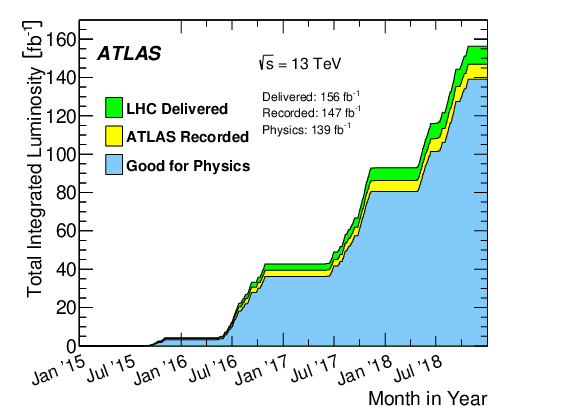
\includegraphics[scale=0.6]{figs/ch3/int_lumi.png}
  \caption{ Cumulative integrated luminosity delivered and recorded by the ATLAS detector during Run 2 of the 
  LHC between the years 2015 to 2018 with a CME of $\sqrt{\textrm{s}}$ = $\textrm{13 \ TeV}$}
\label{fig:3.2}
\end{figure}

Dense proton bunches collide in the \gls{lhc} beam line interaction points, meaning there are multiple \gls{pp} interactions at one time.
Not all interactions are considered and therefore are not saved. Typically, the most energetic collision per bunch crossing, called the hard-scatter,
is analyzed. The symbol denoting the average number of \gls{pp} collisions per bunch crossing is $\upmu$ and is termed pile-up.
The average pile-up for Run 2 is calculated to be $\langle \upmu \rangle$ = $\textrm{33.7}$. The average pile-up over each data taken year of Run 2, along with 
the total average, can be seen in Figure \ref{fig:3.3} \cite{lumi}.

\begin{figure}[h]
  \centering
  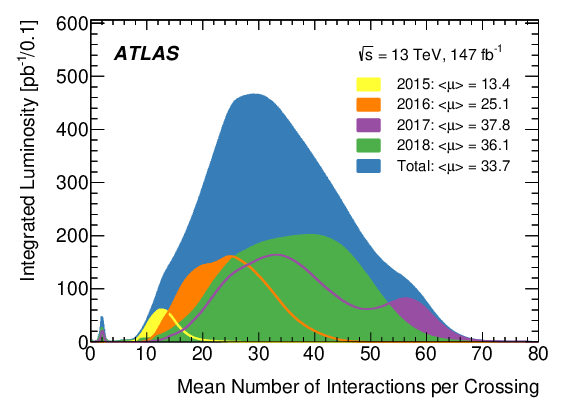
\includegraphics[scale=0.6]{figs/ch3/lumi_weight.png}
  \caption{ The $\upmu$ distribution measured by the ATLAS detector during Run 2 \cite{lumi}}
\label{fig:3.3}
\end{figure}

\section{The ATLAS Detector}

The \gls{atlas} detector is a general purpose detector located 100 meter below \gls{cern} at interaction point 1 on the \gls{lhc} ring.
The purpose of this detector is to probe the \gls{sm} using \gls{pp} collisions and \textit{Nucleus-Nucleus} collisions. Many types of physics 
analyses have been conducted using the \gls{atlas} detector, such as testing predictions for \gls{bsm} within the \gls{sm} as well as precision measurements for 
its physical parameters such as particle mass and lifetimes. The high energies provided by the \gls{lhc} allows physicists to probe very heavy particles such as the 
top quark and the Higgs boson. \gls{atlas} is the largest detector located at CERN. The detector extends 25 meters in height,
44 meters in length and weighs 7000 tons. Figure \ref{fig:3.4} shows an overview of the detector.
\par

\begin{figure}[h]
  \centering
  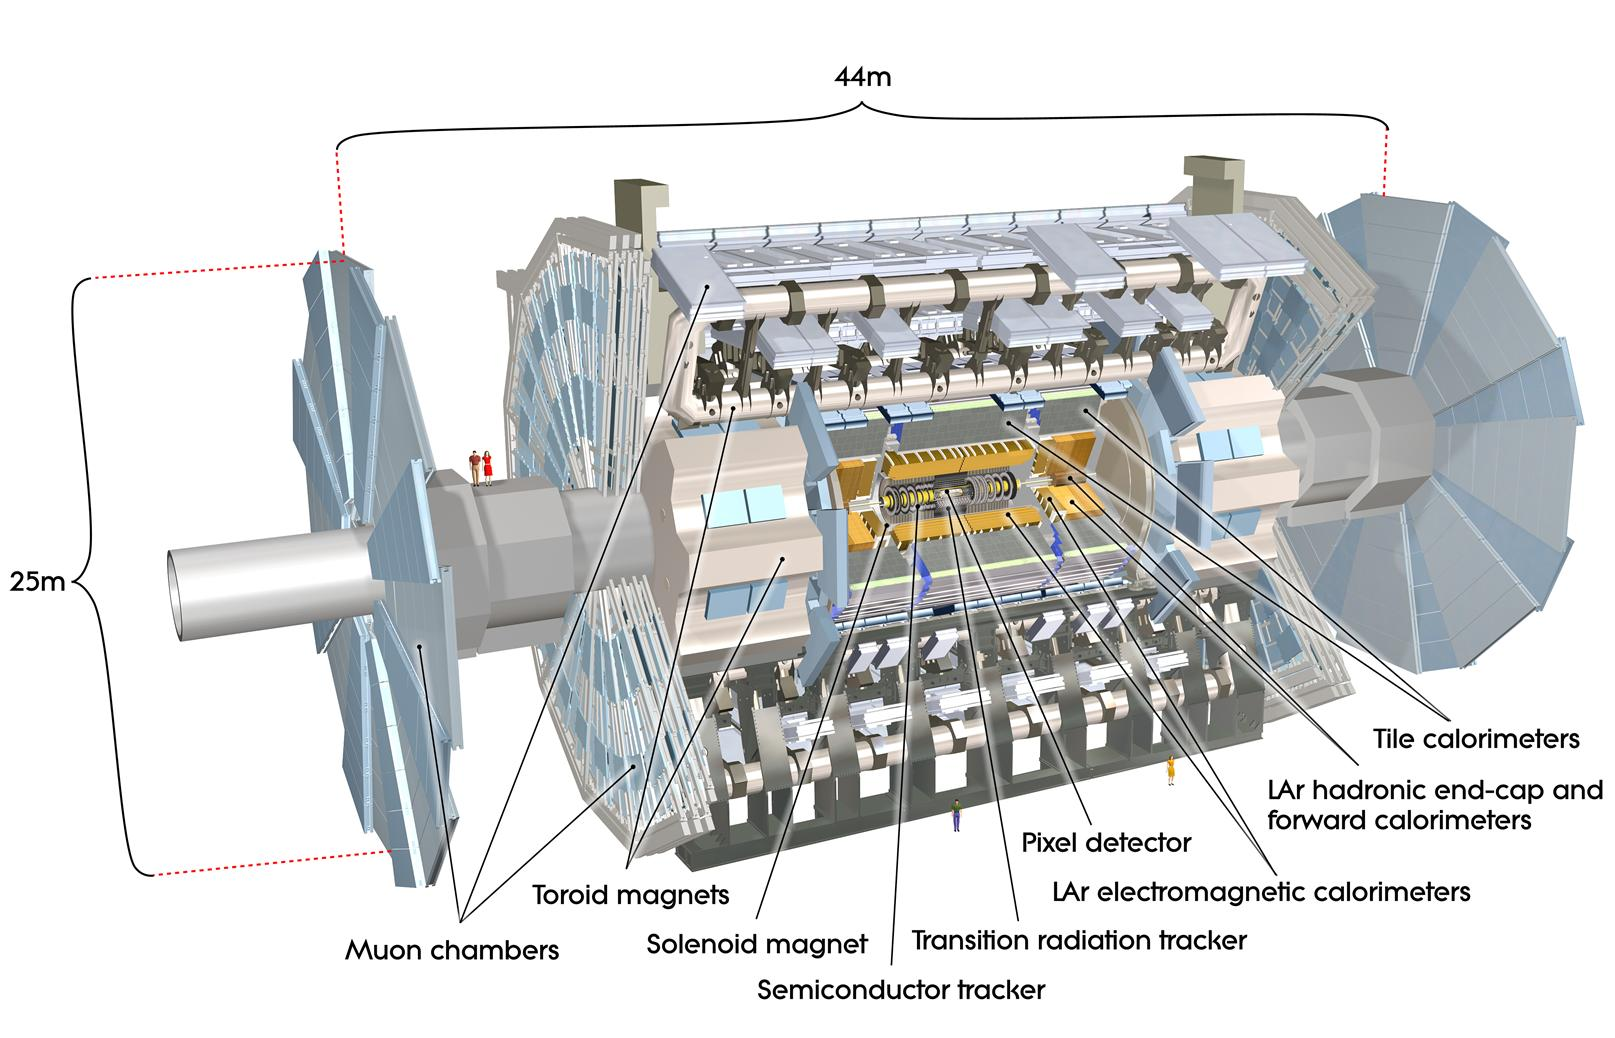
\includegraphics[scale=0.6]{figs/ch3/atlas_run2.png}
  \caption{ The ATLAS detector and its subsystems as of Run 2 \cite{atlas}}
\label{fig:3.4}
\end{figure}

The orange center of Figure \ref{fig:3.4} is the first of the sub-detectors called the Inner Detector (\gls{id}). Approximately 1000 particles are released every 25 ns, therefore high granularity is essential to differentiate the tracks of these particles. The \gls{id} is comprised 
of several parts, pixel and silicon microstrip (\gls{sct}) trackers, these are used in conjunction with the Transition Radiation Tracker (\gls{trt}.).
The \gls{id}'s main goal is to obtain the trajectories and paths of the particles that travel through it. Outside of the \gls{id} is a 
2T solenoid magnet that bends the trajectories of the particles, which allows the momentum to be calculated. After the 2T magnet are the 
calorimeters which function as energy deposition detectors. There are two types of calorimeters used, an electromagnetic calorimeter (\gls{ecal})
in which electrons deposit their energy, the second is called the hadronic calorimeter (\gls{hcal}) where hadrons deposit their energy.
Outside of these two calorimeters is the muon spectrometer (\gls{ms}) which is needed for precise muon momentum measurements. All of these systems 
form a large cylindrical shape around the \gls{lhc} beam pipe. End-caps are placed on the left and right side of the barrel which consist 
of wheel-shaped detectors.

\subsection{The Coordinate System of ATLAS}
\par

A cylindrical and a right-handed Cartesian coordinate system are used in junction within the detector
with the origin placed at the collision point. The x-axis points towards the center of the \gls{lhc}, 
the y-axis points straight up and is used for the basis of the cylindrical coordinate system. The z-axis
points directly down the beam-pipe. Two angles are used to define positions in the detector, the azimuthal angle 
$\upphi$ and pseudorapidity defined as η. Pseudorapidity is defined in Eq. \ref{eq:3.4}:
%
\begin{equation}\label{eq:3.4}
  \textrm{η} = -\textrm{ln}(\textrm{tan}(\frac{\textrm{{θ}}}{\textrm{2}}))
\tag{3.4}
\end{equation}
%
Where θ is the longitudinal angle measured between the z-axis and the trajectory of the particle. Pseudorapidity 
is an approximation of the variable rapidity and is commonly used due to its ease of calculation from the Cartesian
coordinate system and is equivalent to rapidity for massless particles. Rapidity, \textit{y}, is defined as:
%
\begin{equation}\label{eq:3.5}
  \textit{y} = \frac{\textrm{1}}{\textrm{2}}\textrm{ln}(\frac{\textrm{E}+\textrm{\textit{p}}_{\textrm{z}}}{\textrm{E}-\textrm{\textit{p}}_{\textrm{z}}})
\tag{3.5}
\end{equation}
%
Rapidity,  $∆$\textit{y}, is invariant under Lorentz boosts. A benefit of using these variables is that 
η and $\upphi$ provide a Lorentz invariant coordinate system with a distance measurement $∆$\textit{R}, 
defined as: 
%
\begin{equation}\label{eq:3.6}
  ∆\textrm{\textit{R}} = \sqrt{(∆\textrm{η})^{2}+(∆ \upphi)^{2}} 
\tag{3.6}
\end{equation}
%
Due to the physical design of \gls{atlas}, it is impossible to cover the entire η range where highly boosted particles 
are able to leave through the beam-pipe, traveling very close to the z-axis. Table \ref{table:pseudorapidity} shows the total pseudorapidity, η, range 
of all the sub-detectors. 
%
\begin{table}[h]
  \centering 
  \begin{tabular}{ |c |c |}
      \hline
      sub-detector& η coverage\\
      \hline\hline
      Inner Detector  & $\pm$ 2.5 \\
      \hline
      Electromagnetic Calorimeter & $\pm$ 3.2 \\
      \hline
      Hadronic Calorimeter & \\
      Barrel and end-cap & $\pm$ 3.2\\
      Forward Calorimeter & 3.1 < |η| < 4.9\\
      \hline
      Muon Spectrometer & $\pm$ 2.7\\
      \hline
\end{tabular}
\caption{Pseudorapidity of ATLAS sub-detectors \cite{atlas}.}
\label{table:pseudorapidity}
\end{table}

Protons from the collision point only have momentum in the \textit{z}-direction. Therefore the sum 
of the momentum in the transverse plane $\overrightarrow{\textit{P}}_{\textrm{T}} = (\textit{P}_{\textrm{x}}, \ \textit{P}_\textrm{y})^{\textrm{t}}$ 
of particles from the collision point must yield zero. Some particles, such as neutrinos or \gls{bsm} particles,
can escape the detector without depositing energy. The transverse momentum sum of all escaping 
particles can be determined from knowing that the total transverse momentum sum of all escaping particles 
must be zero. If a particle leaves without depositing energy, then the sum of the total transverse 
momentum will be negative and can be shown in the form $\overrightarrow{\textit{P}}_{\textrm{T}}^{\textrm{miss}} = - \sum_{\textrm{detected}}^{\textrm{i}}\overrightarrow{\textit{P}}_{\textrm{T}}^{\textrm{i}}$.
The absolute value of $\overrightarrow{\textit{P}}_{\textrm{T}}^{\textrm{miss}}$ is denoted as $\textrm{\textit{E}}_{\textrm{T}^{\textrm{miss}}}=|\overrightarrow{\textit{P}}_{\textrm{T}}^{\textrm{miss}}|$.
This value is referred to as missing transverse energy (\gls{met}).

\subsection{The Inner Detector}
\par
The \gls{id} consists of three independent sub-detectors that are contained within a cylindrical sleeve with 
measurements of $\pm$3512 mm and a radius of 1150 mm within a solenoid magnet of 2T. The \gls{id} has a pseudorapidity 
range of |η| $\le$ 2.5 and a $\textrm{\textit{p}}_{\textrm{T}}$ threshold of 0.5 GeV \cite{atlas}. 
The \gls{pp} collision points are contained within the \gls{id}. The collision point that contains the highest $\textrm{\textit{p}}_{\textrm{T}}$ is considered the primary vertex. As the decay products travel 
from the primary vertex, after some time, decay themselves, creating a secondary vertex point.
The \gls{id} was uniquely designed to provide robust pattern recognition and momentum resolution
for both primary and secondary vertex measurements for charged particle's tracks. The three sub-detectors provide 
complimentary data acquisition. A decay product is first met by the pixel detector, containing discrete space-points from 
silicon pixel layers. It is then met with stereo pairs of silicon micorstrip (\gls{sct}) layers. Just beyond this is the \gls{trt},
containing many layers of gaseous straw tubes interwoven with transition radiation material. Figure \ref{fig:3.5} shows a layout of the 
\gls{id}, mapping its pseudorapidity coverage and the locations of each sub-detector.

\begin{figure}[h]
  \centering
  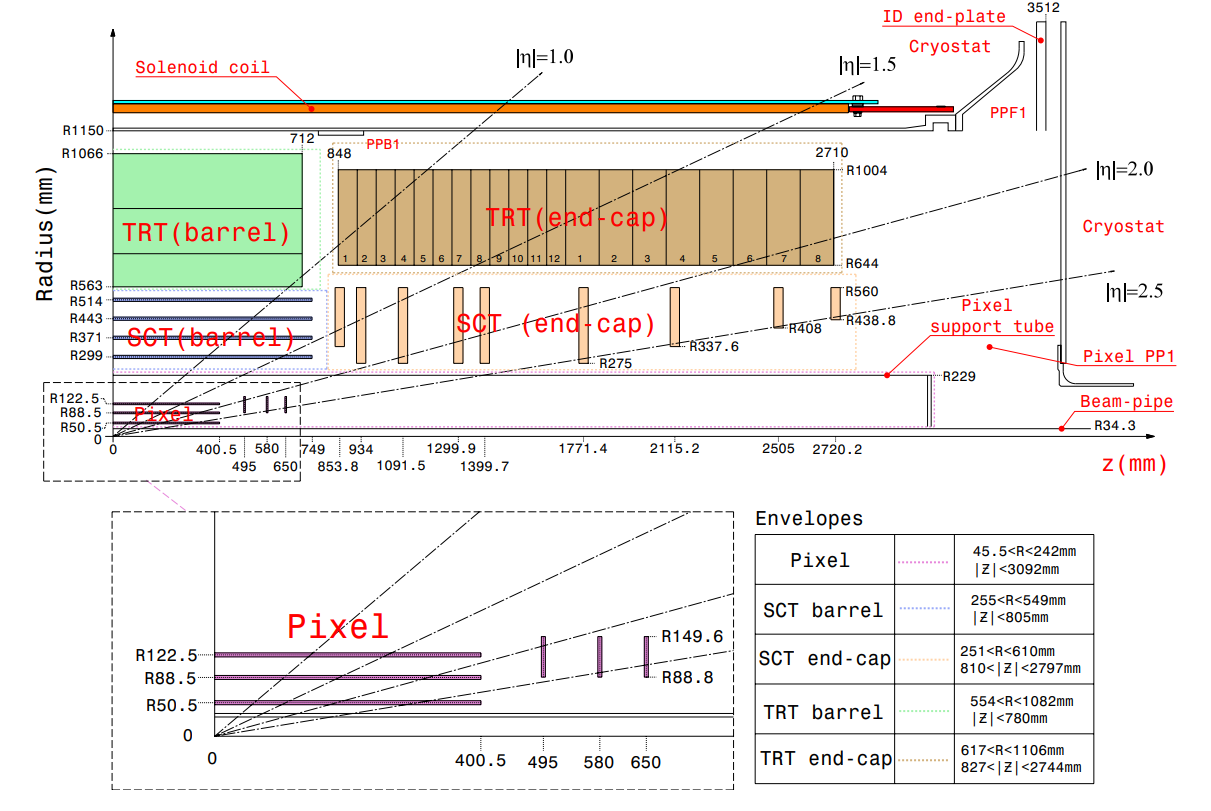
\includegraphics[scale=0.5]{figs/ch3/ID_layout.png}
  \caption{ A quarter-section of the ATLAS ID showing its major elements with their active dimensions. \cite{atlas}}
\label{fig:3.5}
\end{figure}

The \gls{pp} collisions impose a high-radiation environment which require stringent requirements for material composition 
and sensors of the \gls{id} sub-detectors. With the designed life-time of 10 years of operation during Run 2 at the \gls{lhc},
the pixel inner vertexing layer must be replaced every three years. In order to subvert radiation damage over time, the silicon 
sensors are kept at low temperatures, about -5°C to -10°C resulting in coolant temperatures of ~-25°C \cite{atlas}. The \gls{trt}
is kept at room temperature. Figure \ref{fig:3.6} shows a drawing of each sub-detector and their sensors along with a transversed track 
of a charged particle. 

\begin{figure}[h]
  \centering
  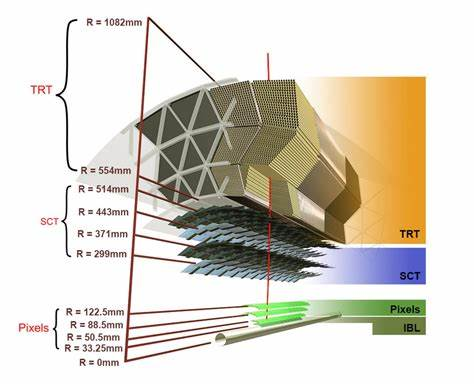
\includegraphics[scale=0.8]{figs/ch3/ID_schem.jpeg}
  \caption{ Drawing of the ID sub-detectors and their sensors. Showing the spacing of each of the sensor layers along with a transversed charged track at η=0.3. \cite{atlas}}
\label{fig:3.6}
\end{figure}

\subsubsection{The Pixel Detector}
\par

The pixel detector consists of three concentric layers of sensors in the \gls{id} barrel and three end-cap discs with sensors
parallel to the transverse plane. The barrel layers are placed at a radii of 50.5 mm, 88.5 mm, and 122.5 mm as shown in Figure \ref{fig:3.6}.
The end-cap discs are located $|\textrm{\textit{z}}|$ = 495 mm$-$650 mm and cover r = 88.8 mm$-$149.6 mm giving an eta coverage 
of $|\textrm{η}| < \textrm{2.5}$. Silicon sensors are pixelated with a pixel pitch of 50$\times$400 µ$\textrm{m}^{\textrm{2}}$ (~90\%) with the remaining being 
50 µm $\times$ 600 µ$\textrm{m}^{\textrm{2}}$. Equaling 47232 pixels per sensor. The short side of the pixel sensors are orientated along $\textrm{\textit{r}}-\upphi$ in both the barrels and the end-caps.
The pixel orientation are 10 µm along the $\textrm{\textit{r}}-\upphi$ and 115 µm in the $\textrm{\textit{z}} \ (\textrm{r})$ in the barrel (end-caps).

\subsubsection{The SCT Detector}
\par
As shown in Figure \ref{fig:3.6}, the \gls{sct} uses silicon strips distributed along four layers in the \gls{id} barrel
and nine discs in each end-cap \cite{atlas}. These layers cover ranges from \textit{r} = 299 mm to \textit{r} = 514
and cover $\textrm{\textit{z}} <$ 749 mm. The end-cap discs are placed at $|\textrm{\textit{z}}|$= 853.8 mm and 
$|\textrm{\textit{z}}|$= 2720.2 mm allowing up to |η| $\le$ 2.5 as seen in Figure \ref{fig:3.7}. The strip modules are rectangularly shaped with 
12 cm strips aligned in the \textit{z}-direction. Trapezoidal strips are implemented in the barrel end-caps. The \gls{sct} strip pitch 
is 80 µm. Three-dimensional coordinates are found by setting two strips back-to-back with an offset of 40 mrad. The intrinsic position 
of the \gls{sct} is 17 µm in the $\textrm{\textit{r}}-\upphi$ and 580 µm in $\textrm{\textit{z}} \ (\textrm{r})$ in the barrel (end-caps)

\begin{figure}[h]
  \centering
  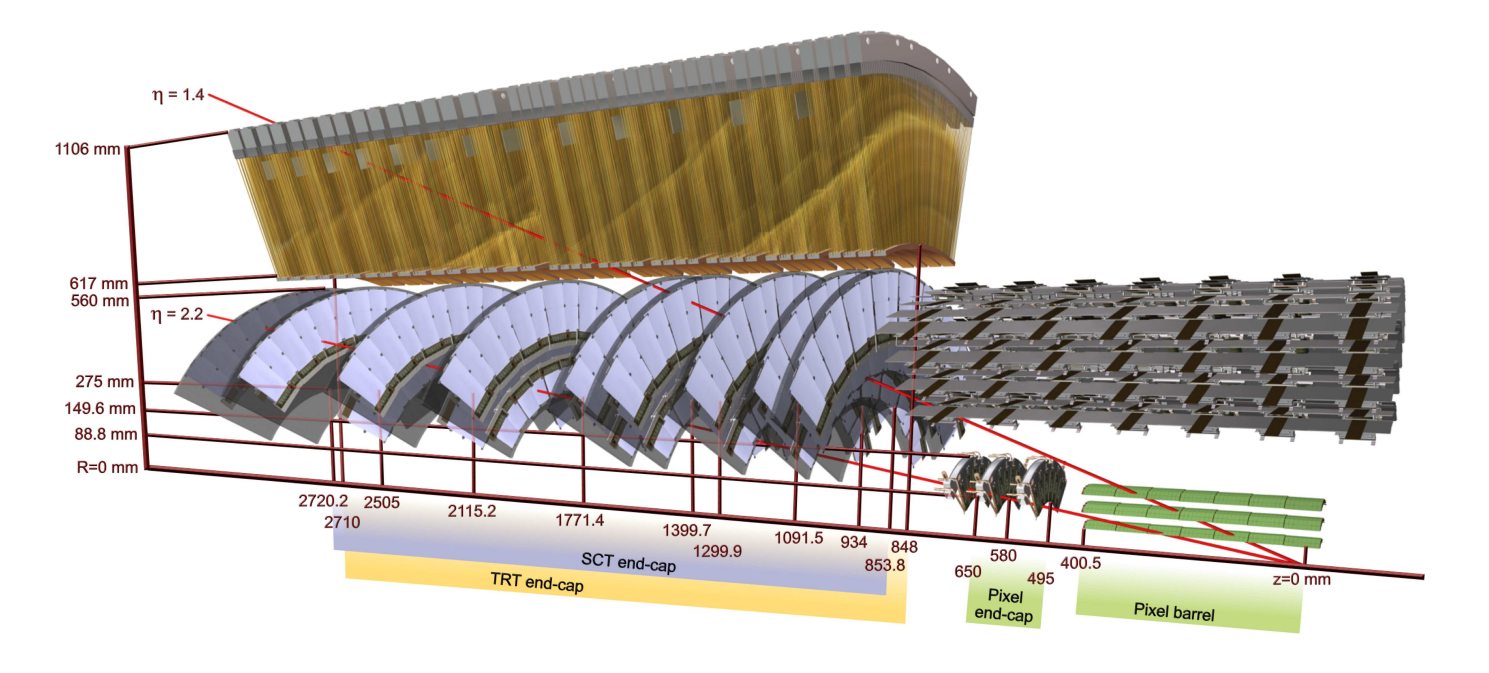
\includegraphics[scale=0.4]{figs/ch3/ID-end-caps.png}
  \caption{  Drawing of the ID sensors of all three sub-detectors and their structural elements focusing on its end-caps transversed by two charged tracks. \cite{atlas}}
\label{fig:3.7}
\end{figure}

\subsubsection{The TRT Detector}

The \gls{trt} is composed of 4 mm diameter polyimide drift straws containing a gas mixture of 70\% Xe, 27\% $\textrm{CO}_{\textrm{2}}$ and 
3\% $\textrm{O}_{\textrm{2}}$ set to 5$-$10 mbar over-pressure. The straws are made of two 35 µm thick multi-layer films bonded back-to-back.
The bare 25 µm thick polyimide film is coated on one side with a 0.2 µm Al layer which is protected by a 5-6 µm thick graphite-polyimide layer \cite{atlas}.
The straws are stabilized using carbon fibers and cut to length of 144 cm for the barrel and 37 cm for the end-caps. For the these drift tubes,
31 µm diameter tungsten anode wires plated with 0.5$-$0.7 µm gold are used and are supported by the straw ends and the end plug. These 
are connected to the electronics and kept at ground potential. Cathodes operate at $-$1530V to give a gain of $\textrm{2.5}\times\textrm{10}^{\textrm{4}}$.
The gas within the straws are ionized as a charged particle interacts with it, releasing drift electrons. These electrons are collected at 
a time of $~$48 ns. The Xe-based gas mixture requires a re-circulating gas system with continuous monitoring of its
quality. The \gls{trt} offers a particle position resolution of 130 µm which is much less than the previous two sub-detectors. The 
\gls{trt} also aids in the identification of charge particles by exploiting transition radiation. 

\subsection{The Calorimeter System}
Surrounding the \gls{id} solenoid are both of the calorimeters that are responsible for measuring charged particles Energy.
Each calorimeter consists of a number of sampling detectors that cover a full $\uppsi$-symmetry and coverage around the beam axis.
The first calorimeter is the \gls{ecal} which detect depositions of electromagnetic particles such as electrons 
and photons. Outside of the \gls{ecal} sits the hadronic calorimeter, its responsible for measuring energy of any hadronic products 
from the collision. Both calorimeter systems use liquid argon as the medium for detecting. These calorimeters have alternate between two 
types of layers, an active layer and a sampling layer. The active layer interacts with charged particles, releasing secondary particles 
that the sampling layer then measures. A calibration is done and converts the deposited energy within the sampling layer to the parent-collision 
particle's energy. 


\subsubsection{Electromagnetic Calorimeters}

\begin{figure}[h]
  \centering
  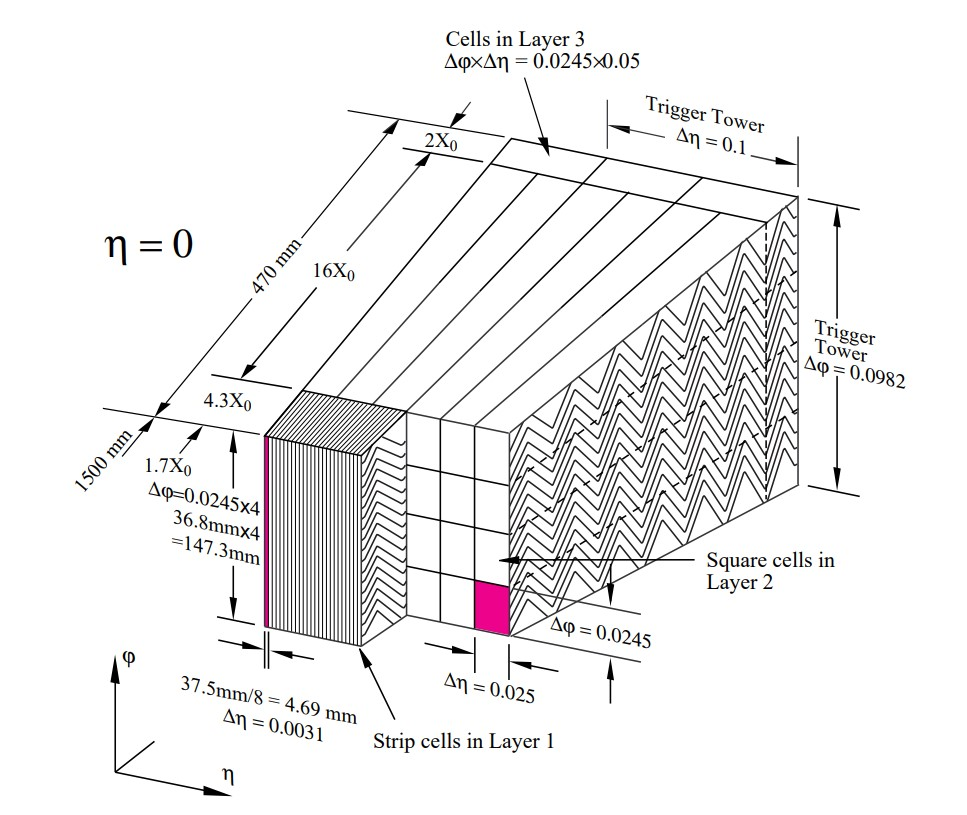
\includegraphics[scale=0.5]{figs/ch3/barrel_module.jpg}
  \caption{  Sketch of a barrel module at η=0. The folds of the electrodes and each layer's granularity is shown \cite{atlas}}
\label{fig:3.9}
\end{figure}
\par

The \gls{ecal} is just outside the solenoid of the \gls{id} and has a barrel shape with two end-caps. Inside this detector are plates
of lead laid inside two sheets of stainless steel that act as an absorber, while liquid-argon acts as the sampling material. Three 
conductive copper layers are located in the gaps between the absorbers and act as electrodes.
These electrodes and absorbers inside this calorimeter are folded in an accordion style. The folding radius varies in length to keep the liquid-argon gap constant. 
Both, the electrodes and absorbers, vary in radius with respect to the liquid-argon gap with the end-caps due to being parallel to the radial 
direction. There are two barrels that cover positive and negative η and are centered at the \textit{z} axis, called the LAr electromagnetic barrel.
One half of the barrel covers $\textrm{0} < \textrm{η} < \textrm{1.475} $ while the second half covers $\textrm{-1.475} < \textrm{η} < \textrm{0}$. The length of 
each barrel is 3.2 m, the inner and outer diameter are 2.8 m and 4 m respectively, weighing a total of 57 tons. Figure \ref{fig:3.9} 
shows a sketch of a barrel module at η = 0 showing each of the three layers and their granularity. 
\par
The end-caps of the \gls{em} calorimeters (\gls{emec}) consist of two wheels, one on each side of the barrels. Each wheel 
is 63 cm thick and weighs 27 tons. These wheels have an η coverage of $\textrm{1.375} < |\textrm{η}| < \textrm{3.2}$. A liquid-argon 
sampler is placed in the region between the wheels of the \gls{emec} and the \gls{ecal} to improve the energy measurement within 
the region which has an η coverage of $\textrm{1.5} < |\textrm{η}| < \textrm{1.8}$. Each \gls{emec} consists of two co-axial wheels located 
in between the inner and outer wheel. These are 3 mm wide and located at $|\textrm{η}|=\textrm{2.5}$.  


\begin{figure}[H]
  \centering
  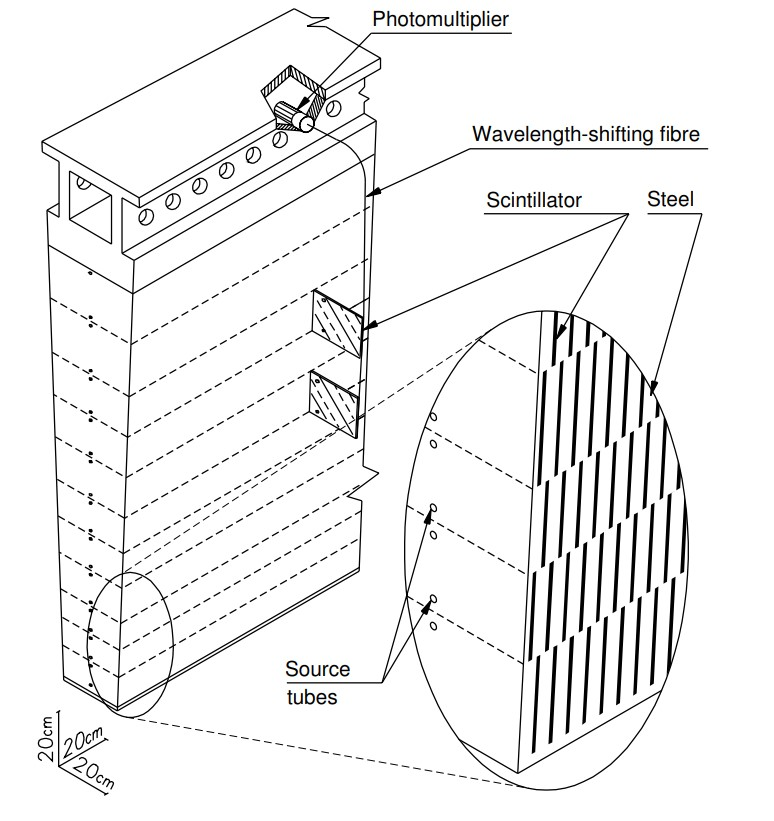
\includegraphics[scale=0.5]{figs/ch3/ecal_section.jpg}
  \caption{  Sketch of the tile calorimeter showing the alternating steel plates and scintillator material attached to PMTs. \cite{atlas}}
\label{fig:3.10}
\end{figure}

\subsubsection{Hadronic Calorimeters}

There are three sub-detectors within the \gls{hcal} system, the tile calorimeter, the liquid-argon hadronic end-cap calorimeter (\gls{hec}),
and the liquid-argon forward calorimeter (\gls{fcal}). The tile calorimeter is a sampling calorimeter that uses steel as the absorber and an 
active medium as a scintillator. It's located just outside the \gls{ecal} and covers an η region of $|\textrm{η}| < \textrm{1.7}$ and is 
divided into three parts, the center barrel extends 5.8 m in length while the two outer barrels extend 2.8 m. The orientation 
of the scintillator tiles are radial and normal to the beam line. 
Attached are wavelength-shifting fibers that extend into readout photomultiplier tubes (\gls{pmt}). A sketch of the tile calorimeter can be 
seen in Figure \ref{fig:3.10}. The output from the \gls{pmt}s are what's recorded. 
\par
The \gls{hec} schematic is shown in Figure \ref{fig:3.11}. This module is an end-cap calorimeter consisting of copper and liquid-argon sampling with 
a flat plate design, cover a range of $\textrm{1.5} < |\textrm{η}| < \textrm{3.2}$. These end-caps share the cryostats with the \
\gls{emec} and the \gls{fcal}. It consists of two wheels in each end-cap, front wheel (HEC1) and the back wheel (HEC2). Each wheel 
contains two longitudinal sections constructed of 32 identical wedge-shaped modules. The \gls{fcal} provide an η coverage of 
$\textrm{3.2} < |\textrm{η}| < \textrm{4.9}$. These modules are located at high η, approximately 4.7 m from the collision point,
exposing them to high particle fluxes. This fact resulted in much smaller liquid-argon gaps to avoid ion build-up and faster signal 
readout. Figure \ref{fig:3.12} shows an illustration of the entire \gls{hcal} section in \gls{atlas}.

\begin{figure}[H]
  \centering
  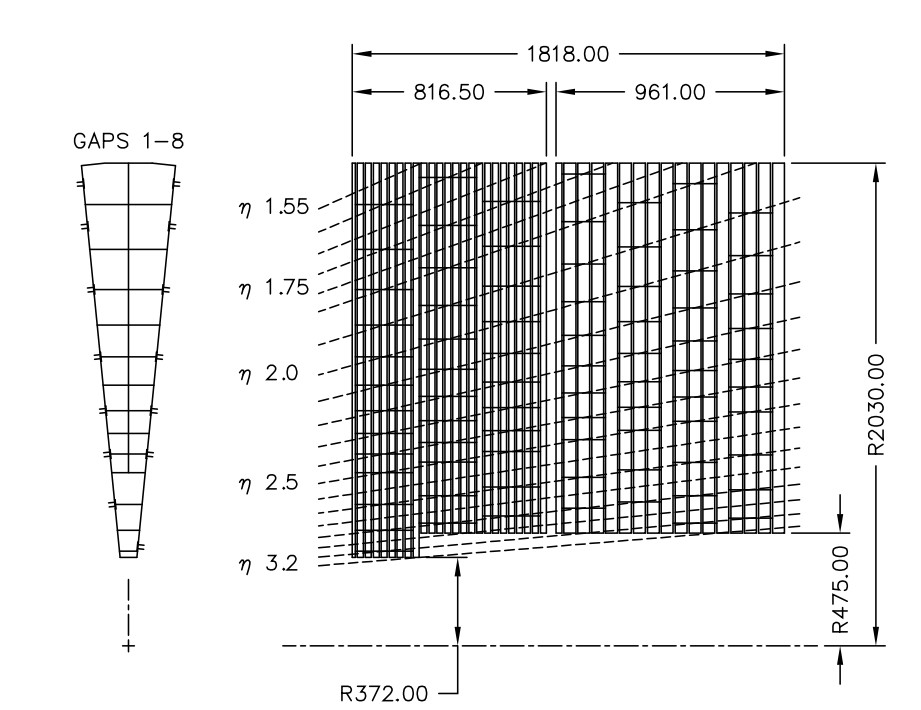
\includegraphics[scale=0.5]{figs/ch3/hcal_barrel.jpg}
  \caption{ Hadronic calorimeter end-cap. Electrode readouts indicated by dashed lines . \cite{atlas}}
\label{fig:3.11}
\end{figure}

\begin{figure}[H]
  \centering
  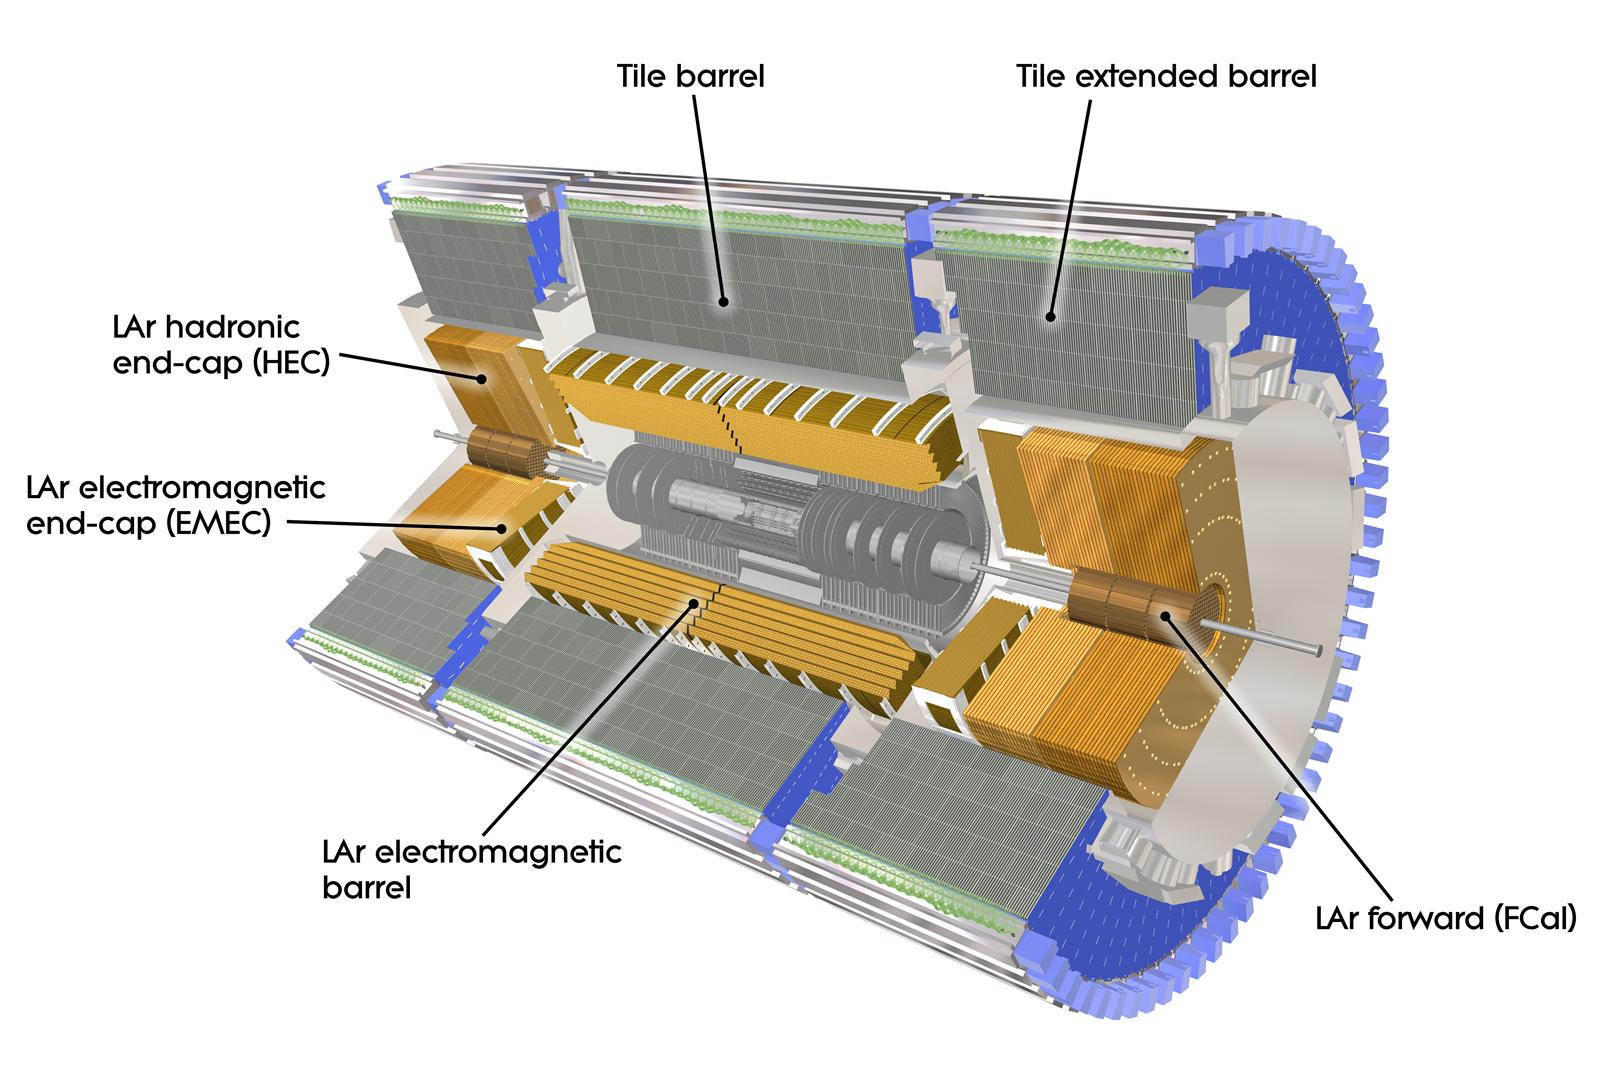
\includegraphics[scale=0.5]{figs/ch3/calorimeters.jpg}
  \caption{  Illustration of the entire HCAL system in ATLAS. \cite{atlas}}
\label{fig:3.12}
\end{figure}

\subsection{The Muon System}

The final system is the muon spectrometer which is designed to detect charged particles exiting the calorimeters 
and to measure their momentum. Muons lose minimal energy when traversing through matter and therefore are depositing minimal energy in 
the \gls{ecal}. The muon system triggers on particles with the pseudorapidity of $|\textrm{η}| < \textrm{2.4}$ and can track up to $|\textrm{η}| < \textrm{2.7}$.
The system consists of three concentric cylindrical shells of gas-filled detectors around the beam axis with radii of 5 m, 7.5 m, and 10 m.
The two end-caps of the muon chambers form large wheels, perpendicular to the \textit{z}-axis and are located 
at $|\textrm{\textit{z}}| \approx \textrm{7.4 m}$, 10.8 m, 14 m and 21.5 m from the collision point \cite{atlas}.
Figure \ref{fig:muon_sys} shows the overall arrangements in two cross-sections of the muon system. The muon trajectories are bent 
using large superconducting toroidal magnets with a generated field mostly perpendicular to the traversing muons.  
\par
The muon gas chambers are filled with 93\% Argon gas and 7\% carbon dioxide, inside the chambers are Monitored Drift Tubes (\gls{mdt}) that perform the precision momentum measurements. The layers consist of three to eight layers 
of \gls{mdt}s and can achieve an average drift resolution 80 µm per tube. In the forward region, $\textrm{2} < |\textrm{η}| < \textrm{2.7}$, Cathode-Strip Chambers (\gls{csc})
are installed within the innermost tracking layer. These are used for their high rate capability and time resolution due to the increase of particle flux. The \gls{csc} have cathodes 
perpendicular to the \gls{mdt}s and the charge induced on the cathode is measured for the signal. The resolution of each chamber is 40 µm in the bending plane (due to the toroidal magnet) and 5 mm in the transverse plane. The muon system is completed with a high precision optical alignment system and is paired with track-based alignment algorithms. 

\begin{figure}[H]
  \centering
  \subfloat[\centering Cross-section of muon system perpendicular to the beam-axis]{{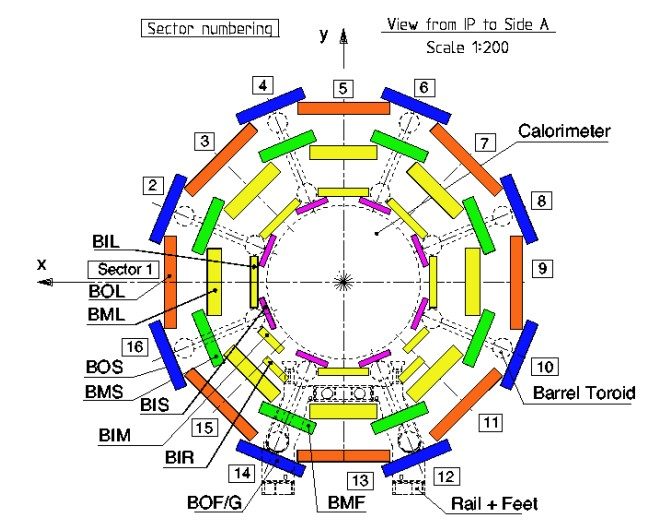
\includegraphics[scale=0.40]{figs/ch3/muon_xsec.jpg}}}%
  \qquad
  \subfloat[\centering Cross-section of muon system in a plane with the beam-axis]{{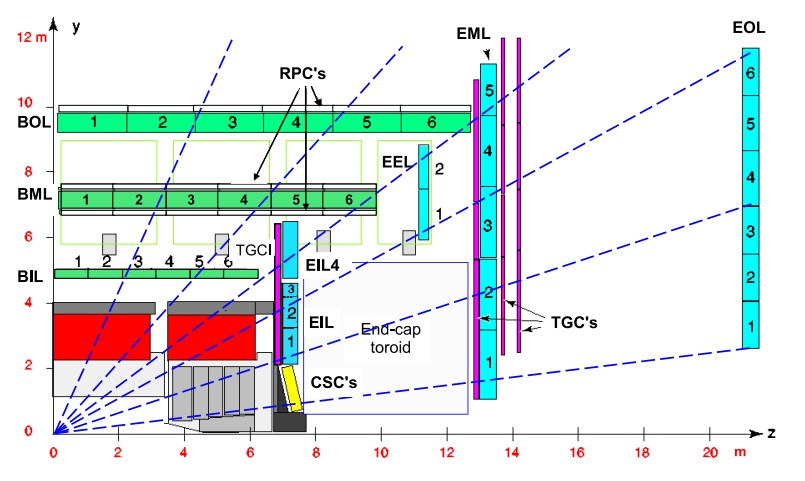
\includegraphics[scale=0.40]{figs/ch3/muon_plane.jpg}}}%
  \caption{Cross-sections of the muon system in the ATLAS detector. Figure (a) shows the three concentric cylindrical layers of 8 large and 8 small chambers. Outer diameter being 20 m. 
  Figure (b) shows a planar view of the muon system, non-bending muon tracks are shown with dashed lines \cite{atlas}}
  \label{fig:muon_sys}
\end{figure}

\subsection{Trigger and Data Acquisition}

\gls{pp} collision rate inside \gls{atlas} occurs at a very high frequency. Bunch crossings occur every 25 ns which equates to a rate of approximately 40 Mhz \cite{atlas}.
The amount of data produced in these \gls{pp} collisions exceeds the storage capabilities, additionally, most bunch crossings feature only low \gls{pp} momentum transfers and 
are therefore not interesting to analyze, let alone store. Therefore a complex selection system is implemented within \gls{atlas} called the Trigger and Data Acquisition (\gls{tdac})
system \cite{trigger}. This system is necessary to only store events that are of interest, reducing the necessity for storage facilities. 
\par
The trigger system consists of three levels of trigger systems. They are Level-1 (L1), Level-2 (L2), and event filter. The L2 and event filter triggers compose the 
High-Level Trigger (\gls{hlt}). The L1 trigger is implemented using custom-made hardware, while the \gls{hlt} is based on the latest software algorithms. The highest 
acceptance rate of the L1 trigger is 75 kHz and the decision making must reach the front-end electronics within 2.5 µs. This trigger mainly searches for signatures from 
high-$\textit{\textit{p}}_{\textrm{T}}$ muons, electrons, photons, jets, $\tau$-leptons that decay into hadrons, and \gls{met} using information collected by the calorimeters and muon 
spectrometer. Figure \ref{fig:3.14} shows a diagram for the L1 trigger. This information is passed to the L2 trigger which reduces the event rate to below 3.5 kHz. The L2 separates this information into Regions-of-Interest (RoI) 
based on coordinates, energy and types of signatures. The event filter uses offline analysis procedures to further reduce the dataset by down to approximately 200 Hz by making decisions 
on fully built events. However, the average acceptance rate of the \gls{hlt} is 1.2 kHz, corresponding to a data rate of 1.2 GB$\textrm{s}^{\textrm{-1}}$ to be written to disc \cite{trigger}. 

\begin{figure}[H]
  \centering
  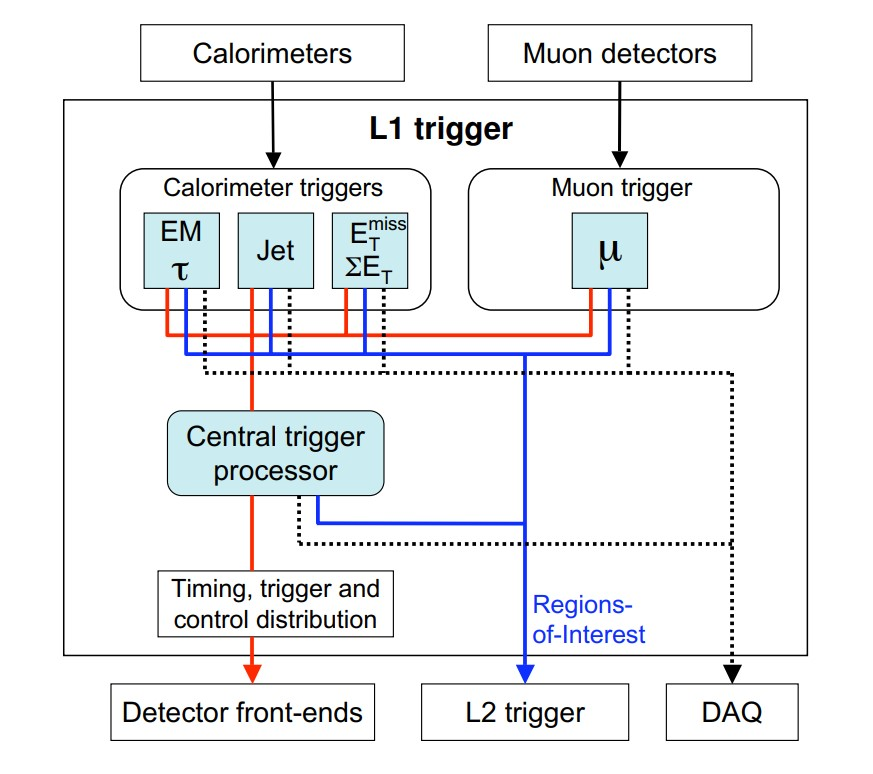
\includegraphics[scale=0.4]{figs/ch3/L1-diagram.jpg}
  \caption{ Block diagram of the L1 trigger in the ATLAS detector showing data paths to the front-end, L2 trigger and DAQs system. \cite{atlas}}
\label{fig:3.14}
\end{figure}

\section{The High-Luminosity LHC and the ATLAS Detector Upgrade}\label{sec:hllhc-itk}

There are two crucial factors in defining rare physics searching capabilities, one is the \gls{cme} and the other is integrated luminosity. The \gls{cme} dictates the 
production cross-section for each physics process, allowing for the produced particle to shift from off-shell (produced at a non-theorized mass) to on-shell (produced at 
theorized mass). Increasing the luminosity equates to increasing the total data production, therefore increasing the amount of rare events one may be looking for. The \gls{lhc} was 
initially designed to run at a \gls{cme} of 14 TeV in which it has obtained a value of 13.6 TeV during Run 3. The current luminosity obtained as been 140 f$\textrm{b}^{\textrm{-1}}$
during Run 2 and an estimated 300 f$\textrm{b}^{\textrm{-1}}$ during the course of the ongoing Run 3. 
\par
The \gls{hllhc} is aimed to fully utilize the capabilities of the \gls{lhc} with a running lifetime of 12 years (called Run 4). It is designed to increase the number of collisions per bunch 
crossing from $\langle \upmu \rangle$ = $\textrm{33.7}$ to $\langle \upmu \rangle$ = $\textrm{200}$. The expected peak luminosity achieved by the \gls{hllhc} is $\textrm{5} \times \textrm{10}^{\textrm{34}} \ \textrm{cm}^{\textrm{-2}}\textrm{s}^{\textrm{-1}}$
The expected integrated luminosity of each year is 250 f$\textrm{b}^{\textrm{-1}}$, with a total of 3000 f$\textrm{b}^{\textrm{-1}}$ after the 12 year run time \cite{hllhc-tech}.
This massive upgrade to the \gls{lhc} requires systems to be upgraded and some to be fully exchanged since these systems are vulnerable to breaking down due to high radiation 
exposure. This increase in radiation is also taken into account within the \gls{atlas} detector, realizing the current infrastructure within the detector is unable 
to withstand this amount of radiation for the running time of Run 4. This high information dense environment now imposes a few new challenges, such as maintaining high 
granularity data readout and the ability for the electronics to maintain this operative power under such high radiation doses. In order to obtain this new feat, the \gls{id} 
will be completely replaced with a new detector sub-system called the Inner Tracker (\gls{itk}) as a part of the \gls{atlas} Upgrade. Part of the work in this thesis 
focuses on preliminary studies of the latest particle identification algorithms implementing the new geometry imposed by the \gls{itk} through computer simulations.

\subsection{The Inner Tracker}

The new tracking detector is designed for a 10 year life span of operation at instantaneous luminosity of 
7.5$\times \textrm{10}^{\textrm{34}}\textrm{cm}^{\textrm{-2}}\textrm{s}^{\textrm{-1}}$, 25 ns per bunch crossing and a total 
integrated luminosity of 3000 f$\textrm{b}^{\textrm{-1}}$ over the entire lifetime \cite{itk-tech}. The current solenoid magnet being used will remain in place and 
provide a magnetic field of 2T as per the previous runs. One of the major improvements (besides being radiation hard) is that the new design will allow 
data collection of quality events of up to $|\textrm{η}| < \textrm{4.0}$. This is achieved through a complex system of silicon barrel layers and disks or rings along with 
inclined pixel modules to have better coverage between the barrel and the end-caps of the \gls{itk}. The barrel will extend $\textrm{η} \approx\pm \textrm{1}$ 
in which the current \gls{id} barrel only has a $\textrm{η} \approx\pm \textrm{0.6}$ coverage.

\subsubsection{ITk Layout}

In the central area in the \gls{itk} barrel, sensors are arranged in cylinders around the beam axis. The first five layers are pixel modules followed by two short-strip layers 
of stereo modules then followed by two even longer strip stereo modules. The forward η regions will be covered using six strip disks on either side and several pixel 
rings. 

\begin{figure}[H]
  \centering
  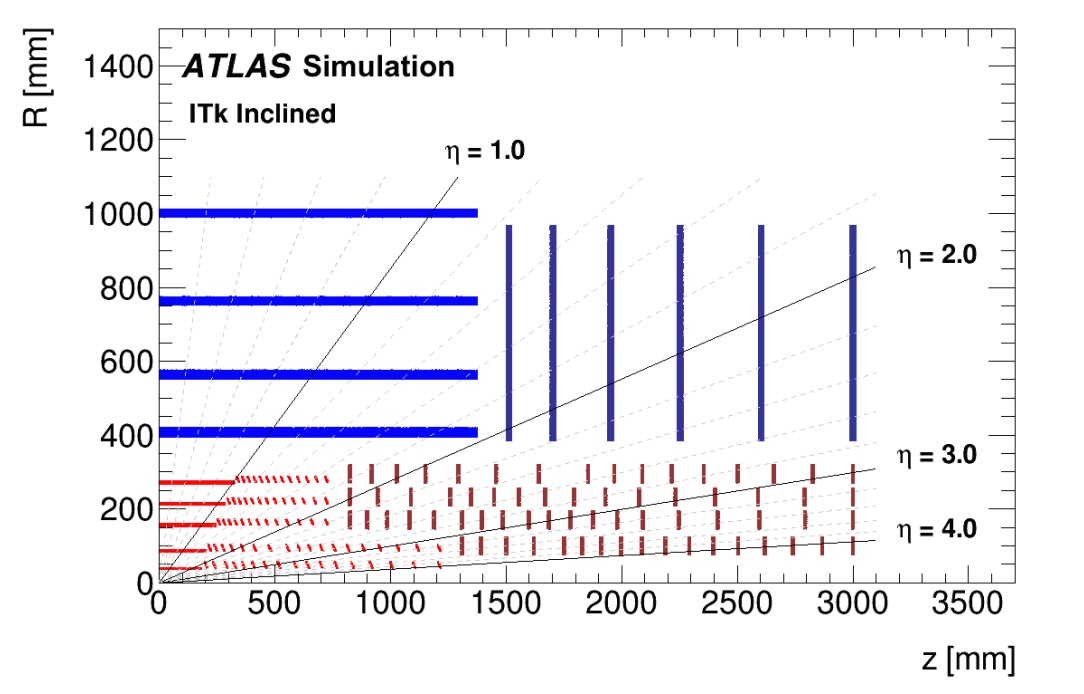
\includegraphics[scale=0.6]{figs/ch3/itk-layout.jpg}
  \caption{ The ITk layout. The pixel detectors are shown in red and the strip Detector in blue.  \cite{itk-tech}}
\label{fig:3.15}
\end{figure}

The strip detectors seen in blue in Figure \ref{fig:3.15} consists of four-layer barrel sections and one end-cap on each side containing six disks. 
This strip system covers $\textrm{η} \approx\pm \textrm{2.7}$ in the barrel region and sits $\pm$ 1400 mm along the \textit{z}-axis. 
The inner layer strips extend a length of 24.1 mm while the outer layer strips are 48.2 mm. All strips within the \gls{itk} have a pitch of 75.5 µm.
Table \ref{table:itk-strip} shows layout parameters of the strip detectors within the detector barrel. 
\par

\begin{table}[t]
  \centering 
  \begin{tabular}{ |c |c |c |c |c |c |}
      \hline
      \multicolumn{6}{|c |}{ITk Barrel Strip Detector Layout Parameters}\\
      \hline\hline
      Layer& Radius [mm]& Channels in $\upphi$& Strip Pitch [mm]& Strip Length [mm]& Tilt Angle [◦]\\
      \hline
      0 & 405 & 28$\times$1280 & 75.5 & 24.1 & 11.5 \\
      1 & 562 & 40$\times$1280 & 75.5 & 24.1 & 11.5 \\
      2 & 762 & 56$\times$1280 & 75.5 & 48.2 & 10 \\
      3 & 1000 & 72$\times$1280 & 75.5 & 48.2 & 10 \\
      \hline
\end{tabular}
\caption{Layout Parameters of the ITk Strip Detector barrel. Each strip is 2.8 m long. \cite{itk-tech}.}
\label{table:itk-strip}
\end{table}

The strips in the six end-cap wheels on each side are radially distributed, pointing towards the \textit{z}-axis. The 
strips vary in length within these end-caps to optimize total strip occupancy, starting at 19.0 mm closer to 
the beam axis, varying up to 60.1 mm in the outermost regions. The exact locations of the end-cap disks and 
strips are shown in table \ref{table:itk-strip-EC}.
\par
Aside from the strip detectors within the \gls{itk}, there are pixel detectors as shown in red in Figure \ref{fig:3.15}. The pixel detector consists of five barrel layers and 
four end-cap ring layers. The layout provides a full eta coverage of  $|\textrm{η}| = \textrm{4}$. The design of the pixel detector allows it to be operating the full lifetime of
12 years. The barrel layer of pixel sensors are placed tangentially of the constant radius of the cylindrical barrel shape. The sensors in the forward parts of the barrel 
are inclined at an angle of 56$^\circ$. Currently, each pixel size is nominally set to 50$\times$50 µ$\textrm{m}^{\textrm{2}}$ with a thickness of 100 µm for the two most inner 
barrel layers and 150 µm for the outer two for simulation. 

\subsection{B-Tagging and Vertex Reconstruction for the ITk}

Event reconstruction is crucial to the integrity of all physics conducted at the \gls{lhc}. In order to effectively reconstruct events, the energy deposition and associated 
tracks must be recorded for the specified event to be rebuilt. As stated earlier, at the \gls{hllhc} it is expected to obtain a pile-up of $\langle \upmu \rangle$ = $\textrm{200}$.
This means the mean separation of primary vertices will be approximately less than 1 mm within the space of the \gls{itk} barrel. Meaning it's not possible for all primary 
vertices of each event to be reconstructed independently. Therefore, it's crucial that all high energetic events coming from a common vertex must be identified to a 
high efficiency. Vertex reconstruction within such an environment imposed strict requirements on tracking resolution close to the particle interaction points. The goal 
is to have reconstructed vertices for $t\overbar{t}$ events to be greater than 0.95 and that the $t\overbar{t}$ decay product is associated to the correct vertex 
at a rate greater than 0.90. The b-tagging versus light-jet rejection should be optimized for each layout and at minimum should match the performance of the \gls{id}.
There is a much more in depth discussion on particle identification and event simulation in chapters~\ref{sec:track-reco} and \ref{sec:event-sim} respectively. 

\subsection{High Granularity Timing Detector}\label{sec:hgtd}

The High Granularity Timing Detector (\gls{hgtd}) is a disc shaped detector that will be placed outside the \gls{itk}. It will be added in front to the end cap and forward calorimeters at 
$|\textrm{\textit{z}}|$= 3.5m. It is composed of two forward and backwards disks with central half rings and stave concepts with a total area of 6 $\textrm{m}^{\textrm{2}}$ of silicon sensors.
The \gls{hgtd} offers a new and powerful technique to overcome the obstacle of pile-up. It takes advantage of the time spread of interactions that occur close in space but spread apart over time. 
This provides a time resolution with a precision measurement of up to 30 ps and will cover an $\textrm{2.4} < |\textrm{η}| < \textrm{4.0}$ where pile-up is rejected \cite{hgtd}.
Figure \ref{fig:3.16} shows the assembly diagram of the \gls{hgtd}

\begin{figure}[ht]
  \centering
  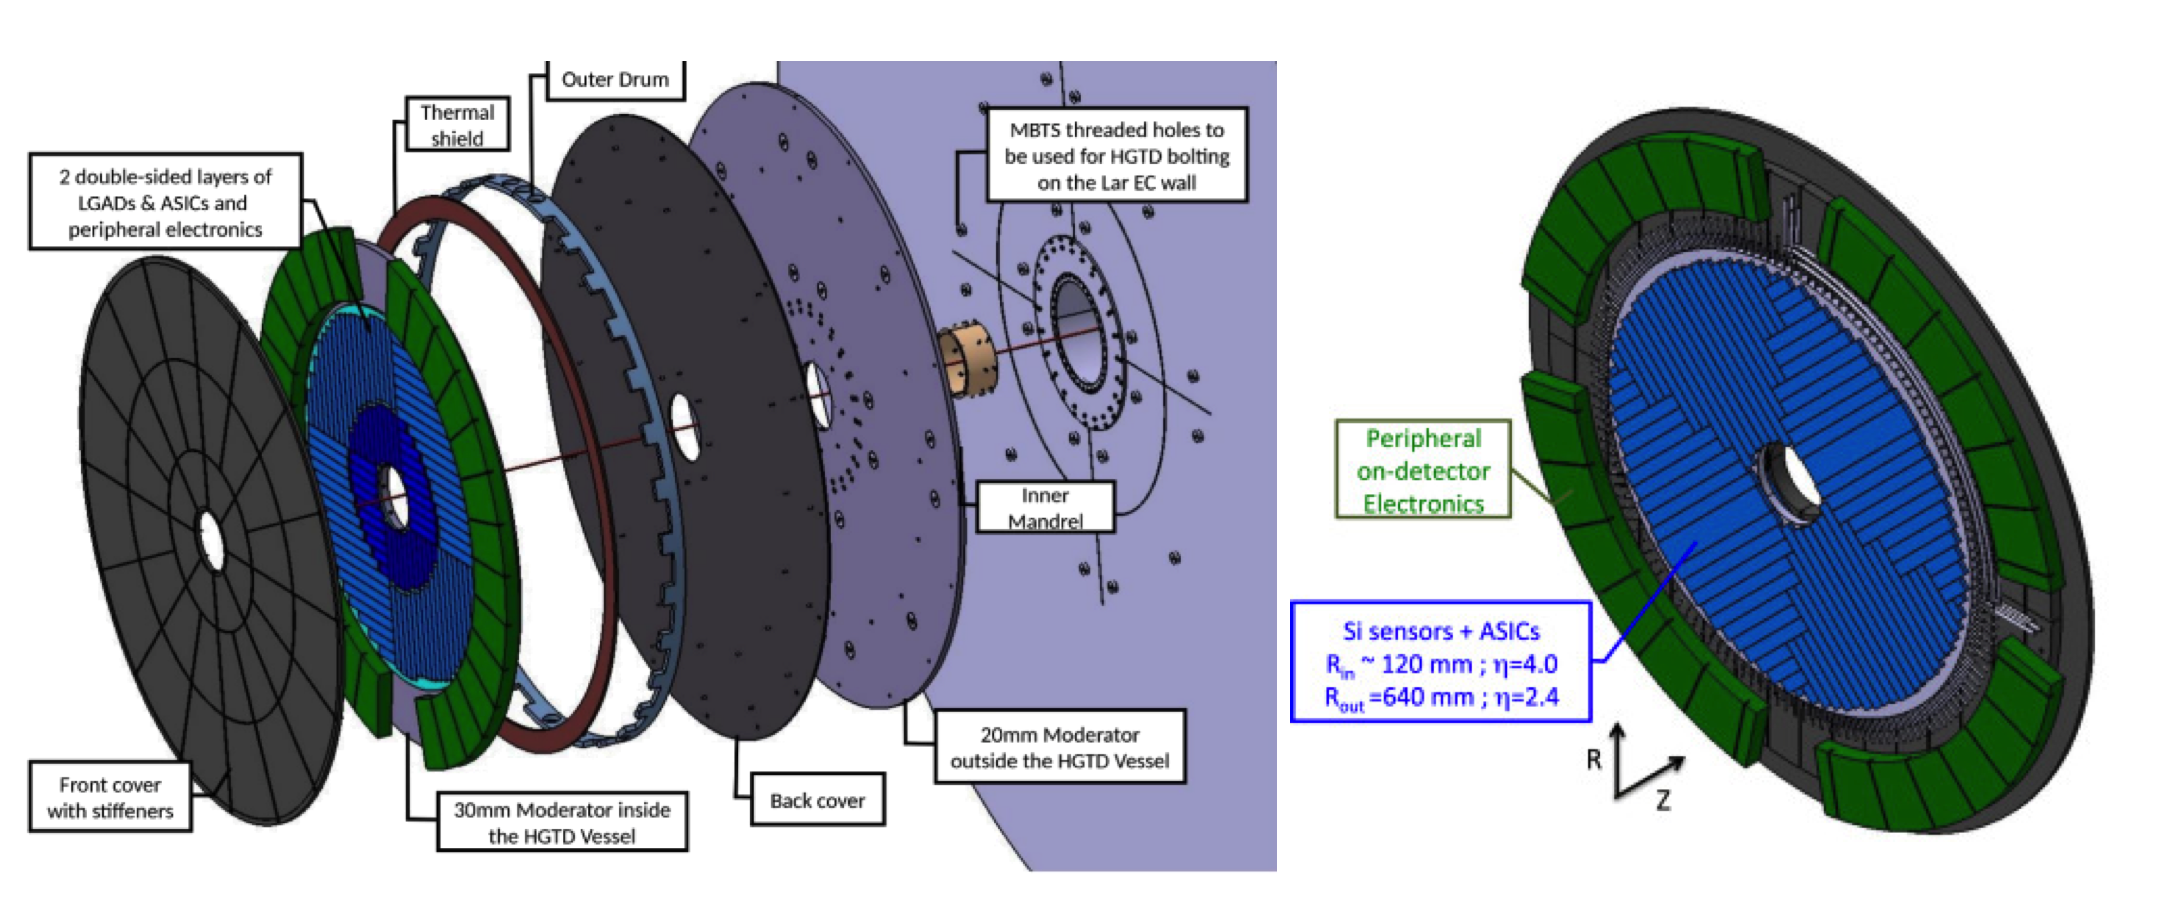
\includegraphics[scale=0.4]{figs/ch3/hgtd_assem.png}
  \caption{ The assembly of the HGTD detector\cite{hgtd}}
\label{fig:3.16}
\end{figure}

The sensors that are built within the \gls{hgtd} are referred to as Low Gain Avalanche Detectors (\gls{lgad}s). 
These sensors will have an active thickness of 50 µm and the pixel area covers 1.3 $\times$ 1.3 $\textrm{mm}^{\textrm{2}}$. The 
sensors will be integrated to an electronic circuit that is currently being developed to meet the requirements of the necessary 
timing resolution and radiation hardness \cite{hgtd}. The \gls{lgad} sensors are n-on-p silicon detectors with an internal gain. 
To obtain this gain, a highly doped, p-layer is added just below the p-n junction. This doped region creates a very high electric 
field and will induce an avalanche of the electrons and thus creating additional electron-hole pairs. Figure~\ref{fig:3.17} shows an illustration 
of the \gls{hgtd}. The blue represents the active \gls{lgad} region and the green is an inactive off-detector region.

\begin{figure}[H]
  \centering
  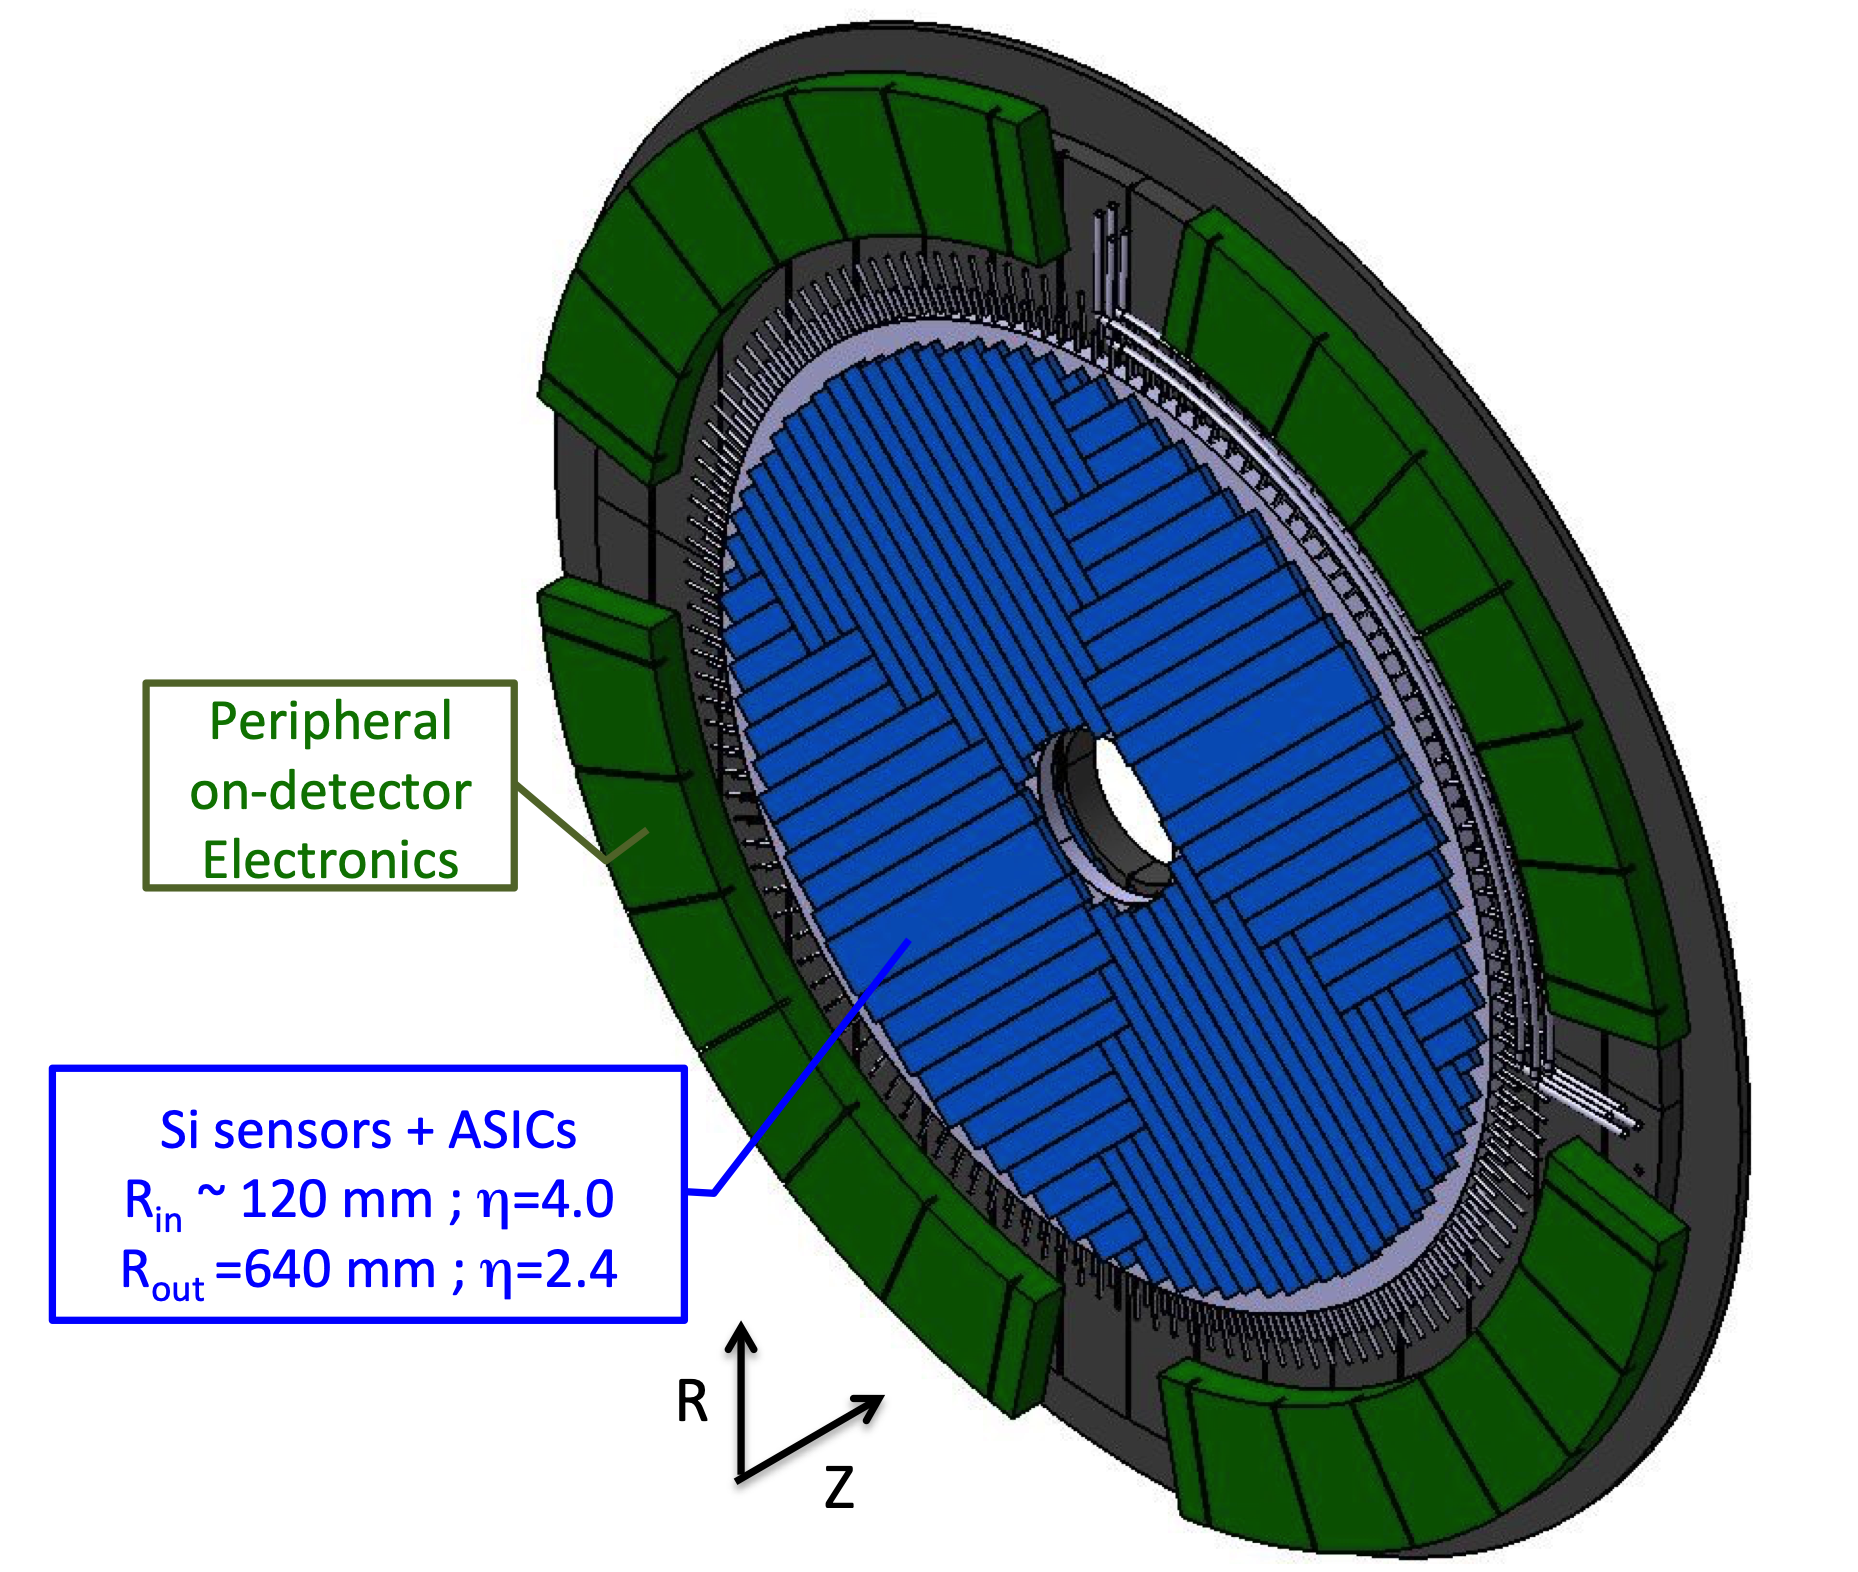
\includegraphics[scale=0.4]{figs/ch3/hgtd_disc.png}
  \caption{ An illustration of the HGTD showing the LGAD sensors (blue) and an inactive region off-detector (green) \cite{hgtd}}
\label{fig:3.17}
\end{figure}

\begin{table}[H]
  \centering 
  \begin{tabular}{ |c |c |c |c |}
      \hline
      \multicolumn{4}{|c |}{ITk Barrel Strip Detector Layout Parameters}\\
      \hline\hline
      Ring/Row & Inner Radius [mm]& Strip Pitch [mm]& Strip Length [mm]\\
      \hline
      Ring 0 Row 0 & 384.5 & 75.0 & 19 \\
      Ring 0 Row 1 & 403.5 & 79.2 & 24 \\
      Ring 0 Row 2 & 427.5 & 74.9 & 29 \\
      Ring 0 Row 3 & 456.4 & 80.2 & 32 \\
      \hline
      Ring 1 Row 0 & 489.8 & 69.9 & 18.1 \\
      Ring 1 Row 1 & 507.9 & 72.9 & 27.1 \\
      Ring 1 Row 2 & 535   & 75.6 & 24.1 \\
      Ring 1 Row 3 & 559.1 & 78.6 & 15.1 \\
      \hline
      Ring 2 Row 0 & 575.6 & 75.7 & 30.8 \\
      Ring 2 Row 1 & 606.4 & 79.8 & 30.8 \\
      \hline
      Ring 3 Row 0 & 638.6 & 71.1 & 32.2 \\
      Ring 3 Row 1 & 670.8 & 74.3 & 26.2 \\
      Ring 3 Row 2 & 697.1 & 77.5 & 26.2 \\
      Ring 3 Row 3 & 723.3 & 80.7 & 32.2 \\
      \hline
      Ring 4 Row 0 & 756.9 & 75.0 & 54.6 \\
      Ring 4 Row 1 & 811.5 & 80.3 & 54.6 \\
      \hline
      Ring 5 Row 0 & 867.5 & 76.2 & 40.2 \\
      Ring 5 Row 1 & 907.6 & 80.5 & 60.2 \\
      \hline
\end{tabular}
\caption{Main layout parameters for the strip detector end-caps. \cite{itk-tech}.}
\label{table:itk-strip-EC}
\end{table}